%  Created by Branden Stone on 2015-01-15.
%  Copyright (c) 2015 Branden Stone. All rights reserved.
%--------------------------------------------------------
\documentclass{article}


%---------------------------
% Packages
%---------------------------
\usepackage{amssymb, amsmath, latexsym, amsfonts, amsthm, mathrsfs} % Standard packages that are nice to have.
\usepackage{amsrefs} % Allows for easy referencing and citations.
\usepackage{verbatim} % Needed for \begin{comment} \end{comment}.
\usepackage[text={6in,9in},centering]{geometry} % Defines the dimensions of the text body.
\usepackage[colorlinks=true]{hyperref} % Allows for use of hyperlinks.
%\usepackage[doublespacing]{setspace} % Makes the document double spaced.
\usepackage[pdftex]{graphicx} % Allows for \includegraphics
\usepackage{enumerate} % Allows for easy modification of lists


%----------------------------
% Title and Author
%----------------------------

\title{Math 390 Homework 2}
\author{Due Wednesday, February 10}
\date{}


%----------------------------
% Main Document Body
%----------------------------

\begin{document}


%-------------------------------------------------------------
% Front Matter: This is where you can add a table of contents,
% preface, list of figures, ETC. for this template we will 
% only create a title and author name with `\maketitle'
%-------------------------------------------------------------

\maketitle

\setlength{\parindent}{0em} % Sets indentation of new paragraph
\setlength{\parskip}{1em} % Sets space between paragraphs

%-------------------------------------------------------------
% Document Body: Essentially this is where you place the 
% content of your document. To use this template, just delete
% all of the text between here and the Bibliography Section.
% Then type whatever you desire.
%-------------------------------------------------------------


Solutions should be written \LaTeX\ or Markdown and converted to a PDF. You are encouraged to work with others
on the assignment, but you should write up your own solutions independently. This means no copy pasting. You should
reference all of your sources, including your collaborators. 

\begin{enumerate}

\item The following graph is called the {\bf Petersen graph}:
	\begin{center}
		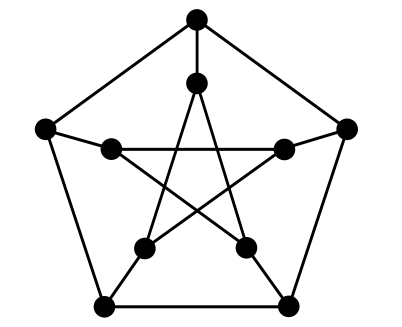
\includegraphics[width=.25\textwidth]{petersen.png}
	\end{center}
Prove (by labeling the vertices) that the graphs below are all isomorphic to the Petersen
graph.
	\begin{center}
		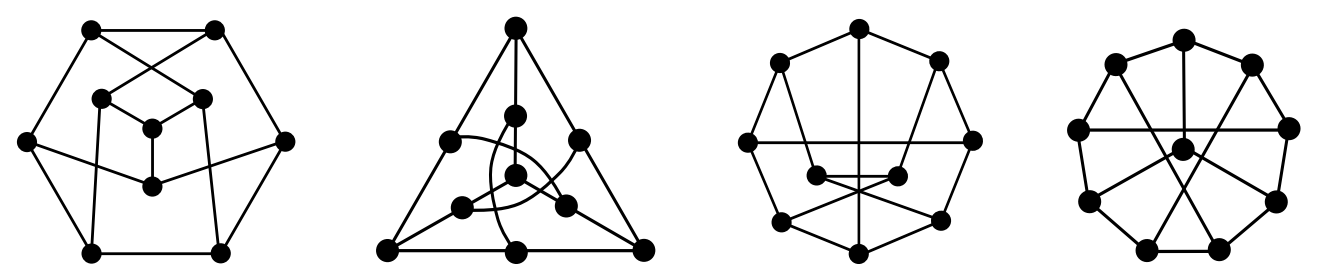
\includegraphics[width=.8\textwidth]{graphs.png}
	\end{center}

\item The \textbf{degree sequence} of a graph is the list of vertex degrees including repetitions.
For each of the following sequences, find a simple graph (no loops or double edges) with
the given degree sequence or prove that no such graph exists.
\begin{enumerate}[(a)]
	\item (1, 2, 2, 3, 4, 5)
	\item (1, 1, 2, 2, 3, 3)
	\item (2, 3, 3, 4, 5, 5)
	\item (3, 3, 5, 5, 5, 5)
\end{enumerate}


\item Suppose that the edges of the graph $K_{17}$ are colored with three colors (red, blue, and
green). Show that the coloring must contain a red triangle, a blue triangle, or a green
triangle.

\item A \textbf{saturated hydrocarbon} is a molecule formed from hydrogen and carbon atoms,
where each carbon atom is bonded to four other atoms, each hydrogen atom is bonded
to one other atom, and no chain of carbon atoms can form a cycle. Consider a saturated
hydrocarbon with $k$ carbon atoms. Prove by induction on $k$ that the saturated
hydrocarbon has exactly $2k + 2$ hydrogen atoms.

\pagebreak

\item 
	\begin{enumerate}
	\item The following picture shows three islands with land on the left and the right. The
	islands and the land are connected by several one-way bridges. Cars can only
	travel on the bridges in the indicated direction. Is it possible to start on the land
	on the left, drive across each bridge exactly once, and end back on the left side?
	Prove your answer. (Hint: Look at Theorem 23.1 in the 4th Edition or Theorem
	2.13 in the 5th Edition of the textbook.)

	\begin{center}
		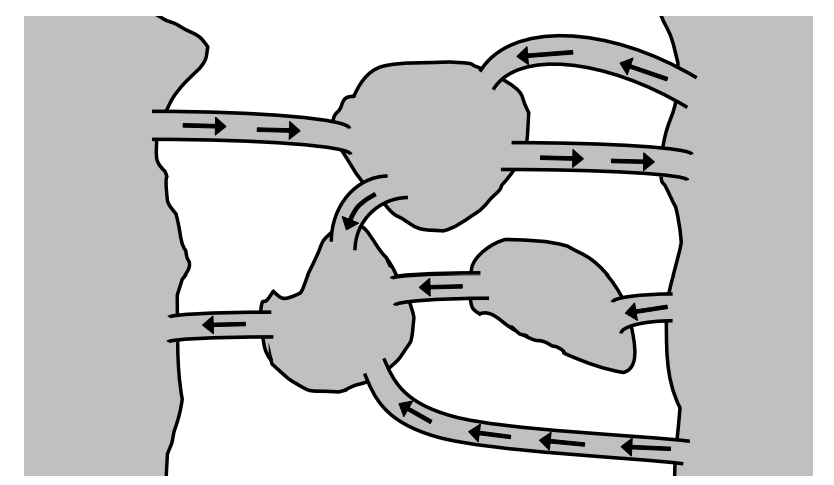
\includegraphics[width=.6\textwidth]{bridge1.png}
	\end{center}


	\item Now, consider the following picture with six islands and land on the left and
	the right. Some of these bridges are one-way, allowing cars to only travel in
	the indicated direction. The bridges without an indicated direction are two-way
	bridges, allowing cars to travel over the bridge in either direction. Is it possible
	to start on the land on the left, drive across each bridge exactly once, and end
	back on the left side? Prove your answer.

	\begin{center}
		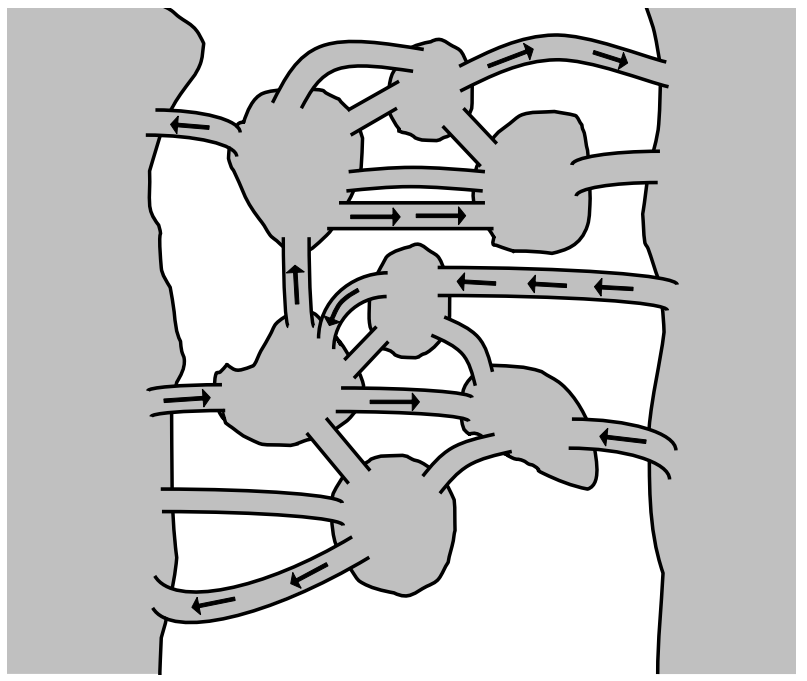
\includegraphics[width=.6\textwidth]{bridge2.png}
	\end{center}
	\end{enumerate}
\end{enumerate}





\end{document}